\subsection{Host-less Cluster SNe~Ia}

As reported in \citet{dawson09a}, we have discovered one potential
host-less cluster SN~Ia among the $8 \pm 1$ cluster SNe~Ia. SN~SCP06C1
is projected near two possible host galaxies: A $z_{850} = 21.6$
spiral galaxy $1''.1$ West of the SN, and a significantly fainter
$z_{850} = 24.6$ galaxy $0''.45$ ($\sim$3.5~kpc at the cluster
redshift) Northeast of the SN (See Fig.~\ref{fig:c1host}).

%%%%%%%%%%%%%%%%%%%%%%%%%%%
% FIGURE: HOST OF SCP06C1 %
%%%%%%%%%%%%%%%%%%%%%%%%%%%
\begin{figure}[tbh]
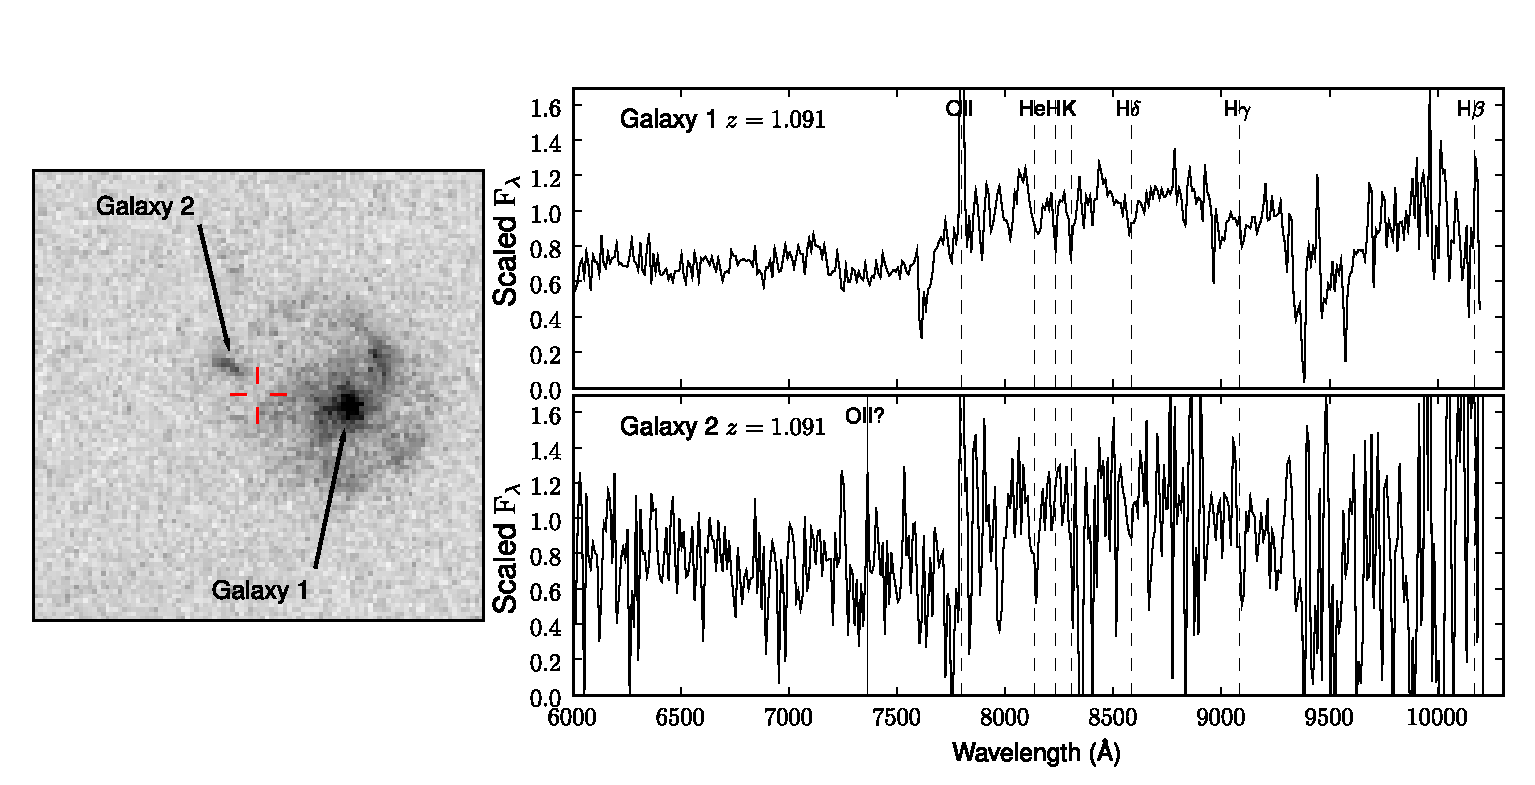
\includegraphics[width=\textwidth]{figures/clrate/SCP06C1_host.eps}
\caption[The environment of SN SCP06C1, a possible intra-cluster
  SN~Ia]{The environment of SN SCP06C1, a possible intra-cluster
  SN~Ia. The red marks show the position of the SN, which has a
  spectroscopic redshift of $z=0.98$, consistent with the cluster
  redshift. The large nearby galaxy (``Galaxy 1'') is at $z=1.091$,
  behind the cluster. The spectrum of the small nearby galaxy
  (``Galaxy 2'') is dominated by light from the larger galaxy -- the
  separation between the two galaxies is only $1''.5$. If Galaxy 2
  were located at the cluster redshift, [O{\sc ii}] would be located
  at the position indicated by ``OII?''\label{fig:c1host}}
\end{figure}

The galaxy-subtracted SN spectrum clearly shows a SN~Ia at redshift
$z=0.98$ near maximum light, consistent with the light curve
fit. The redshift of $z=0.98 \pm 0.01$ is consistent with the cluster
redshift of 0.974.  The bright spiral galaxy is actually in the
background of the cluster, at $z=1.091$. Strong [O{\sc ii}] emission
is visible in the spectrum, along with Ca H \& K and H$\delta$
absorption. Unfortunately, the small separation between the main
galaxy and the smaller galaxy to the Northeast means that the spectrum
of the smaller galaxy is dominated by light from the larger galaxy,
making it impossible to assess a redshift. It is thus possible that
the small galaxy is at the cluster redshift and is the actual host of
the SN. Alternatively, the small galaxy might be at the same redshift
as the larger galaxy and physically associated with it (either as a
satellite galaxy or as part of the spiral structure of the galaxy). It
is interesting to note that the SN is only $20''$ (160~kpc) projected
radius from the center of the cluster, perhaps giving more weight to
the hypothesis that it is associated with a diffuse intracluster
stellar component.

%We might hope to gain insight into the host from the SN parameters. We
%expect the intracluster medium to host an old stellar component. SNe
%occurring in this population would have parameters similar to those in
%passive elliptical galaxies, namely a low stretch value. If the
%stretch were $\gtrsim 1.2$, we might be able to conclude that the SN came
%from a young population \citep[e.g.,][]{brandt10a}. However, the
%stretch of SN SCP06C1 is approximately 1.0 (Suzuki et~al., in
%preparation), which is on the high side of the distribution in passive
%galaxies, but not unusual.

Not being able to confirm or reject this SN as host-less, we have an
upper limit of one host-less SN out of a total of $8 \pm
1$. Discovering one host-less SNe~Ia out of seven total would imply an
intrinsic host-less SN~Ia fraction of $14\% ^{+18\%}_{-7\%}$ (binomial
$68\%$ confidence intervals), and a 95\% upper limit of $<47\%$. This
is broadly consistent with host-less SN~Ia constraints at intermediate
redshifts \citep{sharon10a} and at low redshift
\citep{galyam03a,sand10a}. At low redshift it has been possible to
confirm the host-less nature of some SNe using deeper follow-up
imaging, leading to better constraints. The upper limit of $<47\%$ is
also consistent with direct measurements of intracluster light at low
redshift, but does not strongly constrain evolution. A sample twice
the size or larger, with deeper follow-up to confirm host-less SNe~Ia
would begin to place interesting constraints on hypotheses for the
formation of the intracluster stellar component from $z>1$ to today.

\subsection{Comparison to Other Cluster Rate Measurements}

Cluster SN~Ia rates have been reported at lower redshifts by several
groups. In nearby ($z \lesssim 0.2$) clusters, measurements include
those of \citet{sharon07a} at $z \sim 0.14$, \citet{mannucci08a} at $z
\sim 0.02$, and \citet{dilday10a} at $z \sim 0.09$ and $z \sim 0.22$.
At intermediate redshifts, \citet{sharon10a} recently reported
the rate in $0.5 < z < 0.9$ clusters (median $z \sim 0.6$). At higher
redshifts, \citet{galyam02a} placed the first constraints on the $z
\gtrsim 0.8$ cluster rate using a sample of three clusters at
$z=0.83$, $0.89$ and $z=1.27$.  However, their SN sample included only
one firm SN~Ia at $z=0.83$. The resulting rate has correspondingly
large uncertainties and essentially places only an upper limit on the
$z>0.9$ cluster rate. Our result is thus a large step forward in the
measurement of the SN rate in the highest-redshift clusters.

In Figure~\ref{fig:clrates} we compare our full cluster rate to the
lower-redshift rate measurements that have been normalized by stellar
mass, permitting a comparison across redshifts. Here we have made an
adjustment to the value reported by \citet{sharon10a}. Sharon et
al. used the mass-to-light ratio of Bell03 for the SDSS $g$ and $r$
bands, but did not apply a correction for evolution between $z \sim
0.6$ and $z = 0$.  Using the method described in \S\ref{sec:lum_mass} we
find that a $-0.14$~dex offset should be applied to the mass to
account for evolution from $z=0.6$ to $z=0$ (Fig.~\ref{fig:mlratio},
right panel). We therefore adjust the reported rate of Sharon et
al. upward by 0.14~dex ($38\%$). The rate compilation of \citet{maoz10c}
reflects this adjustment. Whereas the adjusted Sharon et al. rate
shows an indication that the cluster rate is increasing with redshift,
for the first time we find an increasing rate with high significance
($>2\sigma$).

We point out that the popular ``$A+B$'' model \citep{scannapieco05a}
is insufficient for describing the change in cluster rate with
redshift. In the $A+B$ model the SN rate is the sum of a term
proportional to the total stellar mass and a term proportional to the
recent star formation rate: $\mathcal{R}_{\rm SN~Ia} = AM_\ast + B
\dot{M}_\ast$. This simple model is convenient for predicting the SN
rate in environments with varying amounts of recent star formation as
it accounts for the increased SN~Ia rate at short delay
times. \citep[In fact, we use this model in][to derive limits on the
  expected ratio of SNe~Ia to SNe~CC in early-type
  galaxies.]{meyers11a} However, the model lacks theoretical
motivation and breaks down in other situations. For example,
\citet{greggio08a} note that it cannot adequately describe the
observed contribution from SNe with intermediate delay times
\citep[e.g.,][]{totani08a}.  This point is reinforced by the
observation of a changing cluster rate with redshift: In clusters, the
$A$ component is dominant at all redshifts observed. As $M_\ast$ is
not changing significantly with redshift, the rate would be expected
to remain constant under this model. Instead, we require a DTD model
wherein the rate decreases at large delay times (as it does in most
theoretically motivated models).

%%%%%%%%%%%%%%%%%%%%%%%%%%%%%
% PLOTS: CLUSTER RATES, DTD %
%%%%%%%%%%%%%%%%%%%%%%%%%%%%%
\begin{SCfigure}[1.][tbh]
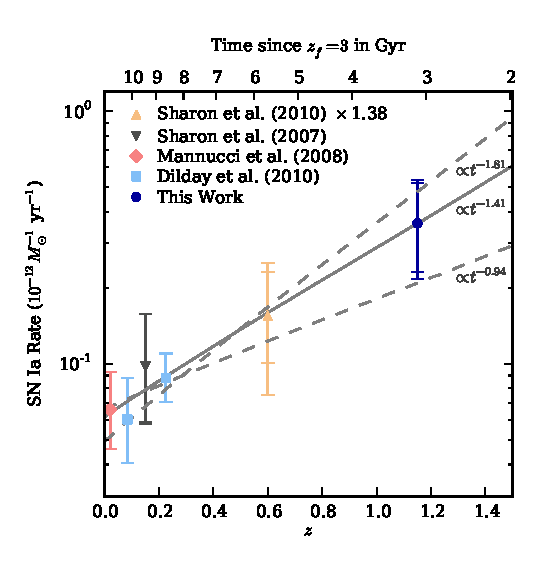
\includegraphics[width=0.6\textwidth]{figures/clrate/clrates_color.eps}
\caption[Cluster rate measurements from this work and the
  literature.]{Cluster rate measurements (all galaxy types) from this
  work and the literature. The rate of \citet{sharon10a} shown has
  been adjusted upward by 38\% from the reported rate (see text). The
  top axis shows the time elapsed since an assumed cluster formation
  redshift of $z_f = 3$. The solid grey line represents the SN
  Ia rate for the best-fit power-law DTD: $\mathcal{R}_{\rm SN~Ia}(t)
  = \Psi(t)/m(t)$, where $\Psi(t) \propto t^s$. The dotted grey
    lines show the range of $1\sigma$ error on $s$.
\label{fig:clrates}}
\end{SCfigure}

\subsection{The Cluster SN~Ia Delay Time Distribution} \label{conclusionsdtd}

The cluster rates constrain the SN~Ia delay time distribution,
$\Psi(t)$, over the range of delay times from a few Gyr to $\sim
10$~Gyr. To illustrate the cluster rate constraints, we parameterize
the DTD with a power law in time: $\Psi(t) \propto t^s$. A power law
is not only a convenient parameterization in the face of limited data,
but is a theoretically motivated function for the DD scenario, where
the late-time ($t \gtrsim 1$~Gyr) DTD shape is set by the distribution
of WD separation after the second CE phase and the merger timescale
due to gravitational radiation \citep{greggio05a}.

We make the approximation that all clusters formed in a single burst
of star formation at $z_f = 3$ and that the age of the stellar
population therefore corresponds to the elapsed time from $z_f$ to the
cluster redshift (Fig.~\ref{fig:clrates}, top axis). While
clearly a simplification, a single star-formation burst captures the
idea that the timescale over which star formation occurred in cluster
early-type galaxies is short compared to the time since star formation
ceased.  The assumed burst redshift $z_f = 3$ is consistent with
measurements of cluster early-type galaxies showing that star
formation was mostly completed by this redshift
\citep[e.g.,][]{gobat08a}. Below, we show that the derived DTD is
relatively insensitive to the redshift assumed.

The DTD is normalized by \emph{initial} stellar mass, whereas the
cluster rate measurements (including ours, for consistency) have been
normalized by \emph{current} stellar mass.  The DTD, $\Psi(t)$, is
therefore related to the cluster rate by $\Psi(t)=m(t)\mathcal{R}_{\rm
  SN~Ia}(t)$ where $m(t)$ is the fraction of stellar mass remaining at
time $t$ after the star formation burst. The specific choice of $m(t)$
does not have a significant impact on the derived DTD: regardless of
the model or IMF assumed, the stellar mass declines by only $\sim$10\%
over the age range of interest, $\sim 3$ to 11~Gyr. For consistency
with \citet{maoz10c}, we use the remaining stellar mass fraction tabulated by
BC03, $m_{\rm BC03}(t)$, but corrected to $m(t) = 1 - (1 - m_{\rm
  BC03}(t))/0.7$ to effectively convert from the Salpeter IMF used in
BC03 to a ``diet'' Salpeter IMF. This correction has only a very small
effect on the result (see below).

We find a best-fit value of
\begin{equation}
s = -1.41^{+0.47}_{-0.40},
\end{equation}
using the statistical$+$systematic error (added in quadrature)
reported for each rate measurement. In Figure~\ref{fig:clrates}, the
solid grey line shows the best-fit cluster rate for this value:
$\mathcal{R}_{\rm SN~Ia}(t)=\Psi(t)/m(t)$, where $\Psi(t) \propto
t^{-1.41}$. Note that the $\chi^2$ of the best-fit model is
surprisingly small: 0.40 for 4 degrees of freedom. The \emph{a priori}
probability of finding a $\chi^2$ smaller than 0.40 is less than
$2\%$. This is difficult to understand given that the measurement
errors are generally dominated by Poisson noise in the number of SNe
observed and are thus unlikely to be overestimated.

The best-fit value is consistent with measurements of the late-time DTD in
the field \citep{totani08a}. Most predictions for the SD scenario show
a steeper late-time DTD \citep{greggio05a,ruiter09a,mennekens10a} with
an effective value for $s$ ranging from $s \sim -1.6$
\citep{greggio05a} to $s < -3$ \citep{mennekens10a}, depending on the
details of the scenario and binary evolution. However, some groups
have found that the SD scenario could be consistent with a less-steep
DTD ($s \sim -1$) given the right combination of main sequence and red
giant secondaries \citep{hachisu08a}.  In the DD scenario, the
predicted shape of the DTD depends on the distribution of binary
separations after the common envelope phase of the WDs, a difficult
distribution to predict. However, a slope of $s = -1.4$ (and a range
of similar values) would not be surprising in the DD scenario.

\subsection{Additional DTD Systematic Uncertainties} \label{conclusionssys}

Variations in the assumed cluster star formation, initial mass
normalization and mass-to-light ratio evolution have a small affect on $s$
compared to the measurement error.

(1) \emph{Age of clusters' stellar populations:} Above, we assumed a
single burst of star formation at $z_f = 3$. Moving this single burst
to $z_f = 4$ results in $s = -1.55$. A more recent burst, $z_f = 2.5$,
results in $s = -1.30$.  \citet{maoz10c} give a treatment of variations from
the single-burst approximation, also finding that the affect on $s$ is
small.

Our rate measurements in red and early-type galaxies provide a good
consistency check that recent star formation does not significantly
contribute to the SN~Ia rate: if it did, we would observe a higher
rate in the full cluster than in these subsamples. Surprisingly, we
observe the opposite trend (although the significance is low). The
red-sequence early-type subsample includes 53\% of the stellar mass of
the full cluster sample, and 6 SNe~Ia. The remaining 47\% of the full
cluster sample (which includes bluer galaxies and late-type
red-sequence galaxies) accounts for only $2 \pm 1$ SNe~Ia. At low
redshift, \citet{mannucci08a} found a similar trend between E/S0
galaxies and S0a/b galaxies within $0.5$~Mpc of cluster centers,
though also at $<1\sigma$ significance.

(2) \emph{Remaining stellar mass:} Whereas the DTD is normalized by
initial stellar mass and cluster rate measurements have been
normalized by current stellar mass, we have assumed a remaining
stellar mass fraction $m(t)$ to convert from current to initial
stellar mass. Although different models and IMFs can yield significantly
different $m(t)$, we are only concerned here with the change in $m(t)$
between $\sim 3$~Gyr and at $\sim 11$~Gyr. (The absolute value of
$m(t)$ affects only the normalization of $\Psi(t)$, with which we are
not concerned.) Fortunately, the evolution in $m(t)$ in this age range
is small and consistent between models, and so the effect on $s$ is
small. For example, using $m_{\rm BC03}(t)$ (assuming a Salpeter IMF)
rather than correcting to a diet Salpeter IMF (as we have done) only
changes the best-fit value from $s=-1.41$ to $s=-1.38$.

If in \S\ref{sec:lum_mass} we had used a $M/L$ ratio directly
normalized by initial mass, rather than normalizing by current mass
and later converting to initial mass, the results would be very
similar. (We have not done this for consistency with other rate
measurements.) In the {\sc p\'egase2} models in
Figure~\ref{fig:mlratio} (left panel) evaluated at $z=1.2$, the ratio
of current to formed stellar mass varies slightly across the models,
but is fully contained in the range $0.66 \pm 0.03$. The same models
evaluated at $z=0$ have a ratio of $0.59 \pm 0.03$. This is consistent
with the $\sim 10\%$ evolution in $m(t)$ over this range as tabulated
by BC03.

(3) \emph{$M/L$ ratio evolution:} While the overall normalization of
the $M/L$ ratio will only affect the normalization of $\Psi(t)$ and
not $s$, the evolution of the $M/L$ ratio will affect $s$. In
\S\ref{sec:lum_mass} we assigned a liberal 20\% systematic uncertainty to
the evolution of the $M/L$ ratio over the redshift range of
interest. To estimate the effect of this systematic uncertainty, we
adjust our rate measurement by 20\% and that of \citet{sharon10a} by
10\% and refit $s$. The resulting change in $s$ for positive and
negative shifts is $-0.15$ and $+0.18$ respectively, less than half of
the nominal error in $s$.

%Our measurements of the SN~Ia rate in red-sequence and red-sequence
%early-type galaxies help constrain the possible impact of SNe from
%younger stellar populations. One concern for the interpretation of the
%DTD above is that the assumption of a negligible amount of recent star
%formation is not valid. This is a particular concern for
%higher-redshift clusters where we are closer to the epoch when most of
%the stars are formed.  Given that the SN~Ia rate is orders of
%magnitude higher a short time after star formation, even a small
%amount of younger populations could contribute significantly to the SN
%rate, biasing our measurement. Our rate measurements in red and
%early-type galaxies provide a good consistency check: Were there a
%significant contribution to the full cluster rate from younger stellar
%populations, we would observe a lower rate in these subsamples.
%However, even in subsets of galaxies within narrow bounds of the red
%sequence (Fig.~\ref{fig:ratevscut1}) and in the ``most elliptical''
%galaxies (Fig.~\ref{fig:ratevscut2}), we see a rate consistent with
%the full cluster rate. This is consistent with measurements in
%lower-redshift clusters showing a similar contribution to the rate
%from early- and late-type galaxies \citep{mannucci08a} and gives us
%confidence that the cluster rate can be used at even higher redshifts
%to constrain the DTD in the future.


%Maoz10 use our cluster SN~Ia
%rate in combination with the lower-redshift cluster rates, cluster
%iron abundances, and various other rate measurements in order to
%constrain the DTD over a wide range of delay times.


%For an additional illustration, we also
%compare the cluster rates to one numerical DTD from the literature
%\citep{mennekens10a} in Figure~\ref{fig:dtd}. Here, both the DD and SD
%curves have been scaled up by a factor of 10 to match the low-redshift
%cluster rates. The rates thus constrain the shape of the curves, not
%the overall amplitude.

%\begin{figure}
%\epsscale{1.175}
%\plotone{figures/clrate/dtd.eps}
%\caption{Cluster rate measurements compared to the numerical DTD
%  models of \citet{mennekens10a}. As in Figure~\ref{fig:clrates}, a
%  cluster formation of $z_f = 3$ is assumed. Both the DD and SD curves
%  have been scaled up by a factor of 10 to match the low-redshift
%  cluster rates. \label{fig:dtd}}
%\end{figure}

%Although the results seem to rule out a significant contribution from
%the SD scenario, we must be careful in our interpretation,
%particularly concerning the stellar ages assumed. Here we have assumed
%that all stars form at $z_f=3$ and that there is no star formation
%after. If in reality, there were a low level of ongoing star formation
%up to $z=0$, a DTD steeper than $t^{-1.5}$ could be interpreted as
%being much less steep.




